\chapter[Simulazione del preamplificatore]{Simulazione di reti di condizionamento per la lettura di SiPM}
I segnali in uscita dal SiPM non hanno un'ampiezza tale da essere apprezzati dalla MuonPi Board. È quindi necessario utilizzare un circuito detto 
preamplificatore il più vicino possibile al SiPM per evitare di amplificare rumore. Il preamplificatore deve avere le seguenti caratteristiche:
\begin{itemize}
    \item amplificare il segnale in uscita dal SiPM di circa \SI{20}{\dB};
    \item fornire la tensione di polarizzazione al SiPM;
    \item AC-coupling dell'input del preamplificatore.
    \item avere una tensione di alimentazione di circa \SI{5}{\volt}.
\end{itemize}\cite{muonpiwikicontributors_2017_sipm}
Una possibile soluzione per la realizzazione di un circuito che rispetti i vincoli appena elencati si basa su un dispositivo di tipo commerciale chiamato 
BGA614. Quest'ultimo è prodotto dall'azienda Infineon Technologies e rientra nella tipologia di ciruciti integrati detti MMIC (Monolithic 
Microwave Integrated Circuit), che operano cioè a frequenze dell'ordine delle microonde (da \SI{300}{\mega\hertz} a \SI{300}{\giga\hertz}). 
Il BGA614 è l'elemento circuitale che garantisce al circuito un guadagno di circa \SI{20}{\dB} a frequenze pari a \SI{1}{\giga\hertz} ed è 
ottimizato per corrente di ingresso tipiche di \SI{40}{\milli\ampere} \cite{infineontechnologiesag_2011_bga614}. Dal punto di vista circuitale si compone, come mostrato nella 
\autoref*{fig:bga614_circuito}, di due transistor BJT, di cui il $Q_1$ della figura in configurazione emitter follower.
\begin{figure}[h!]
    \centering
    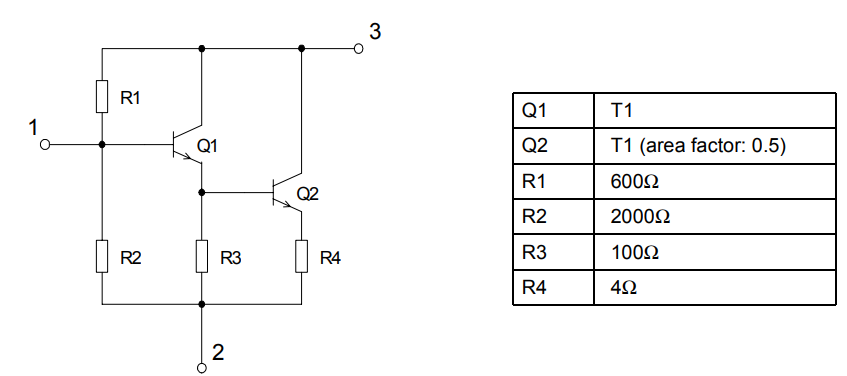
\includegraphics[width=1\linewidth]{img/bga614_circuito.png}
    \caption{Schema circuitale del BGA614. I pin 1 e 3 vanno collegati al circuito mentre il pin 2 va collegato a massa.}
    \label{fig:bga614_circuito}
\end{figure}
Si osserva che i due transistor BJT sono in una configurazione simile a quella di Darlington (\autoref*{fig:darlington_configuration}) eccezion 
fatta per la resistenza $R_3$, facendo intuire quindi un comportamento simile. In questo tipo di circuiti, la corrente $I_C=\beta_\text{EQ}*I_B$, 
dove $\beta_\text{EQ}=\beta_1 \cdot \beta_2+\beta_1+\beta_2$. Si tratta quindi di un amplificatore. Uno svantaggio di questa configurazione è quello
di avere una tensione $V_{\text{BE}} = V_{\text{BE}_1} + V_{\text{BE}_2}$, quindi una tensione di soglia maggiore rispetto a quella che si avrebbe 
con un solo transistor. Altro svantaggio risiede nel fatto di avere un tempo di risposta minore.
\begin{figure}[h!]
    \centering
    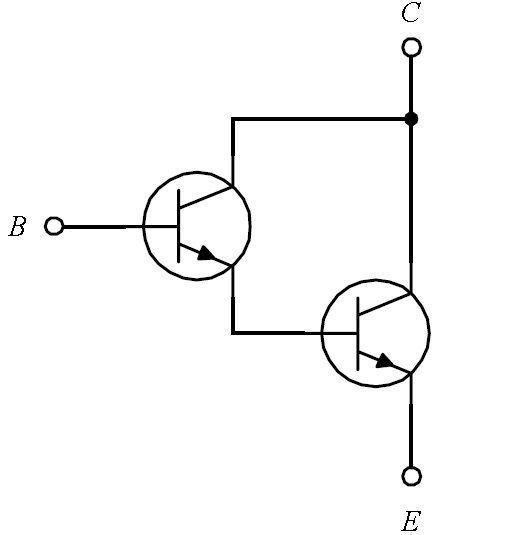
\includegraphics[width=.325\linewidth]{img/darlington_configuration.jpg}
    \caption{Schema circuitale della configurazione Darlington \cite{david_2019_}.}
    \label{fig:darlington_configuration}
\end{figure}

Considerando quanto detto fino ad ora, l'intero circuito di preamplificazione è quello che appare nella \autoref*{fig:preamp_circuito}.
\begin{figure}[h!]
    \centering
    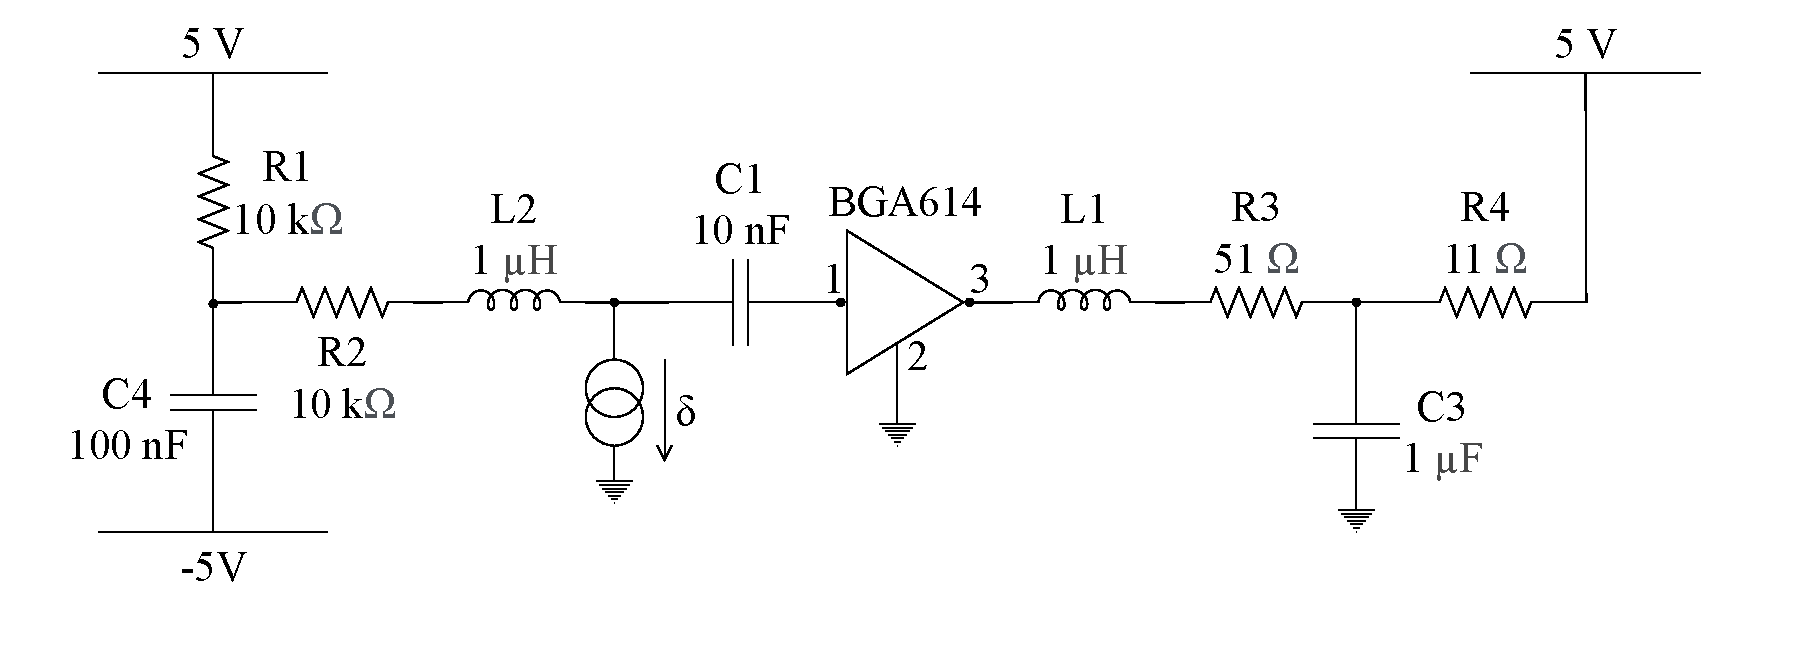
\includegraphics[width=1\linewidth]{img/preamp_circuito.pdf}
    \caption{Schema circuitale del preamplificatore. Il generatore di corrente $\delta$ è il modello del sottosistema SiPM-scintillatore.}
    \label{fig:preamp_circuito}
\end{figure}
Per comprendere a meglio il funzionamento del circuito, si è deciso di simularlo usando il programma LTSpice e di risolverlo mediante l'uso di 
equazioni. Per poter simulare il circuito con LTSpice è sufficiente inserire nello schematico, presente all'apertura del programma, i componenti del circuito 
con i loro valori, che in questo caso si trovano sullo schematico fornito dal progetto MuonPi, e scegliere il tipo di simulazione da effettuare. 
A questo punto, il programma creerà un file chiamato \texttt{netlist} nel quale sono presenti tutte le direttive per la costruzione e
la simulazione del circuito. Nel caso preso in esame si è interessati alla simulazione del punto di lavoro stazionario, del comportamento di piccolo segnale e della risposta in 
transitorio, quest'ultima necessaria per capire come il circuito si comporta all'arrivo del segnale a gradino proveniente dal sensore costituito da 
scintillatore e SiPM. Per risolvere matematicamente il circuto, invece, occorre effettuare due tipologie di analisi: l'analisi delle componenti 
stazionarie (punto di lavoro stazionario) e l'analisi delle componenti di segnale in frequenza (analisi di piccolo segnale).
Per risolvere il punto di lavoro stazionario per circuiti con all'interno transistor BJT sono necessarie una serie di assunzioni per non 
rendere i calcoli estremamente complessi. Per esempio, si assume normalmente che la tensione tra base ed emettitore $V_{\text{BE}}$ sia pari a 
\SI{0,6}{\volt}. Assunzioni come la precedente causano la generazione di una serie di approssimazioni che a cascata rendono i calcoli teorici 
leggermente diversi dai risultati simulati, dato che quest'ultimi tengono conto delle equazioni complete.
Per questo motivo verranno riportati i soli calcoli svolti per l'andamento di piccolo segnale che verranno poi analizzati insieme a quelli ottenuti  
dai calcoli, mentre per l'analisi del punto di lavoro verranno presi in considerazione solo i riultati ottenuti dalla simulazioni.
\section{Punto di lavoro stazionario}
L'obiettivo del calcolo del punto di lavoro stazionario è quella di ottenere il valore in continua di tutte le correnti che scorrono nei rami del circuito 
e di tutte le tensioni ai nodi e stabilire se il circuito in questa condizione sia acceso o spento. Per esempio, nel caso di circuiti 
contenenti BJT, come quello analizzato ora, si richiede una tensione tra collettore e emettitore $V_{\text{BE}}>\SI{20}{\milli\volt}$.
Per fare ciò, bisogna considerare i soli generatori di tensione e corrente in continua, considerando come cortocircuiti i generatori di
tensione alternata e come circuiti aperti i generatori di corrente alternata. Inoltre, si cortocircuitano gli induttori e si trasformano in 
circuiti aperti i condensatori. Dopo queste operazioni, il circuito appare come quello della \autoref*{fig:preamp_circuito_pdl}.
\begin{figure}[h!]
    \centering
    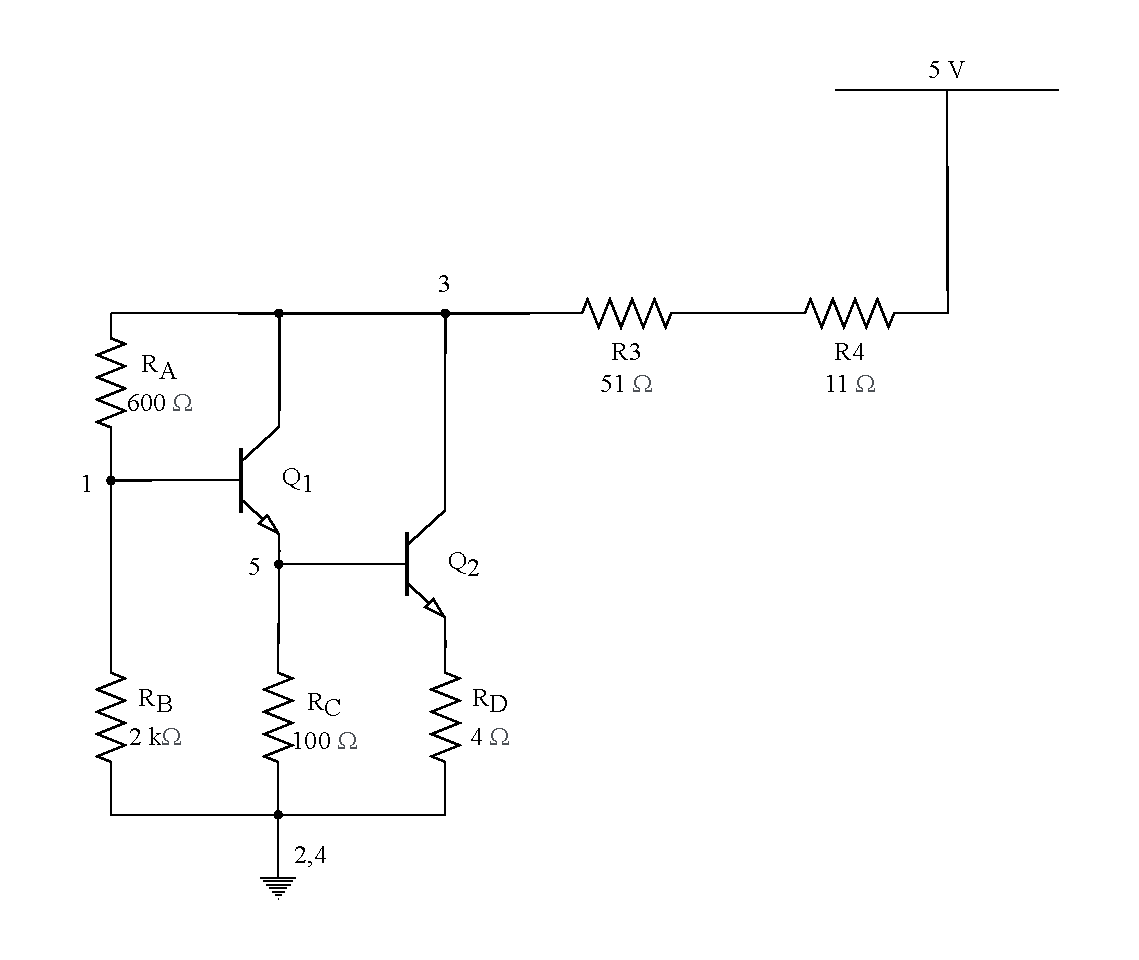
\includegraphics[width=1\linewidth]{img/preamp_circuito_pdl.pdf}
    \caption{Schema circuitale del preamplificatore in DC.}
    \label{fig:preamp_circuito_pdl}
\end{figure}
Per simulare il punto di lavoro stazionario utilizzando LTSpice è sufficiente la direttiva \texttt{.op}. I risultati della simulazione si trovano
all'interno di un file di log e sono riportati nella \autoref*{tab:pdl_results}, mentre nella \autoref*{tab:pdl_results_bjt} sono riportati i 
valori delle grandezze elettriche proprie dei transistor BJT $Q_1$ e $Q_2$.
\begin{table}[ht!]
    \centering
    {\renewcommand{\arraystretch}{1.3}
        \begin{tabular}{cc}
            \toprule
            Tensione        & Valore                        \\
            \midrule                                
            $V_3$                      & \SI{2,52}{\volt}           \\
            $V_1$                      & \SI{1,80}{\volt}           \\
            $V_5$                      & \SI{0,99}{\volt}           \\
            \bottomrule
        \end{tabular}
    }
    \caption{Valori delle tensioni nel punto di lavoro stazionario.}
    \label{tab:pdl_results}
\end{table}
\begin{table}[ht!]
    \centering
    {\renewcommand{\arraystretch}{1.3}
        \begin{tabular}{ccc}
            \toprule
            Parametro             & $Q_1$                         & $Q_2$                        \\
            \midrule                                
            $I_C$                 & \SI{10,62}{\milli\ampere}     & \SI{28,21}{\milli\ampere}    \\
            $I_B$                 & \SI{0,30}{\milli\ampere}      & \SI{0,98}{\milli\ampere}     \\
            $V_\text{BE}$         & \SI{0,80}{\volt}              & \SI{0,88}{\volt}             \\
            $V_\text{CE}$         & \SI{1,52}{\volt}              & \SI{2,40}{\volt}             \\
            $\beta$               & $34.90$                       & $28.80$                      \\
            $g_m$                 & \SI{0,37}{\per\ohm}           & \SI{0,912}{\per\ohm}         \\
            \bottomrule
        \end{tabular}
    }
    \caption{Valori delle correnti, delle tensioni e delle transconduttanze dei due BJT.}
    \label{tab:pdl_results_bjt}
\end{table}
Facendo riferimento al circuito nella \autoref*{fig:preamp_circuito_pdl}, sono rilevanti principalmente i valori
di tensione del nodo 3, ai valori delle due transconduttanze $g_m$ e ai valori di tensione tra collettore e emettitore $V_\text{CE}$ nei due transistor.
In particolare si vede che per entrambi i transistor $V_\text{CE}>\SI{20}{\milli\volt}$, perciò si deduce che entrambi i transistor sono in 
regione attiva diretta, amplificando così la corrente applicata sulla base secondo l'equazione $I_C=\beta \cdot I_B$, dove $\beta$ è detto guadagno
di corrente ed è proprio di ogni transistor. Sostituendo i valori di $\beta$ e $I_B$ presenti nella \autoref*{tab:pdl_results_bjt}, è possibile 
verificare se l'equazone $I_C=\beta \cdot I_B$ è corretta o si tratta di una approssimazione eccessiva. Dalla \autoref*{tab:confronto_bjt} 
emerge un errore relativo bassissimo, perciò la formula per il calcolo della $I_C$ è molto coerente con quanto avviene nella simulazione.
\begin{table}[ht!]
    \centering
    {\renewcommand{\arraystretch}{1.3}
        \begin{tabular}{cccc}
            \toprule
            Grandezza elettrica   & Valore simulato               & Valore calcolato              & Errore relativo  \\
            \midrule                                
            $I_C(Q_1)$            & \SI{10,62}{\milli\ampere}   & \SI{10,60}{\milli\ampere}   & $\SI{0,12}{\%}$ \\
            $I_C(Q_2)$            & \SI{28,22}{\milli\ampere}   & \SI{10,24}{\milli\ampere}   & $\SI{0,07}{\%}$ \\
            \bottomrule
        \end{tabular}
    }
    \caption{Confronto tra valori simulati e valori calcolati.}
    \label{tab:confronto_bjt}
\end{table}
\section{Analisi di piccolo segnale}
L'obiettivo dell'analisi di piccolo segnale è di trovare la funzione di trasferimento che lega la tensione presente nel nodo di ingresso 
alla tensione presente nel nodo di uscita. Per fare ciò, occorre trasformare tutte le grandezze elettriche
presenti nel circuito nel loro equivalente nel dominio delle frequenze: i generatori di corrente continua diventano dei circuiti aperti,
i generatori di tensione continua diventano dei cortocircuiti e, nel caso del circuito preso in analisi, ogni transistor BJT in regione attiva diretta
viene sostituito da un generatore di corrente tra il collettore e l'emettitore, il cui valore è dato dall'equazione $i_c=g_m \cdot v_\text{be}$.
Il modello per descrivere il BJT è quello utilizzato nei calcoli svolti e vale sotto due approssimazioni: si suppone $\beta\to \infty$ e si suppone 
una corrente di collettore indipendente dalla tensione tra collettore e emettitore $V_\text{CE}$. La potenza di calcolo del simulatore permette, 
invece, di usare un modello più complesso per il BJT che non tiene conto delle approssimazioni appena descritte. Così facendo occorre inserire due 
resistenze: una tra base ed emettitore $r_\pi=\frac{\beta}{g_m}$ e una tra collettore e emettitore in parallelo al generatore di 
tensione $r_\text{ce}=\frac{V_\text{AF}+V_\text{BC}}{I_C}$, dove $V_\text{AF}$ è la tensione di Early diretta che assume generalmente valori da 
alcune decine ad alcune centinaia di volt \cite{graffi_2007_transistori}. Nella \autoref*{fig:bjt_ac_model} si vede la differenza circuitale tra i due modelli. A questo punto, il circuto di cui 
viene fatta la risoluzione mediante equazioni è modellizzato dalla \autoref*{fig:preamp_circuito_ac}.
\begin{figure}[h!]
    \centering
    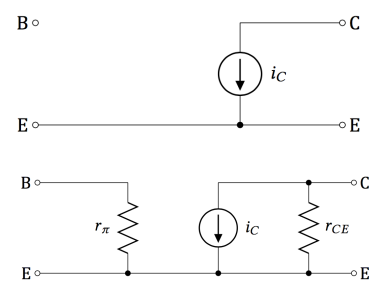
\includegraphics[width=.65\linewidth]{img/bjt_ac_model.png}
    \caption{In alto il modello in AC del BJT in cui vengono considerate le approssimazioni, sotto il modello usato dal simulatore senza
     approssimazioni, con la presenza delle due resistenze $r_\pi$ e $r_\text{ce}$.}
    \label{fig:bjt_ac_model}
\end{figure}
\begin{figure}[h!]
    \centering
    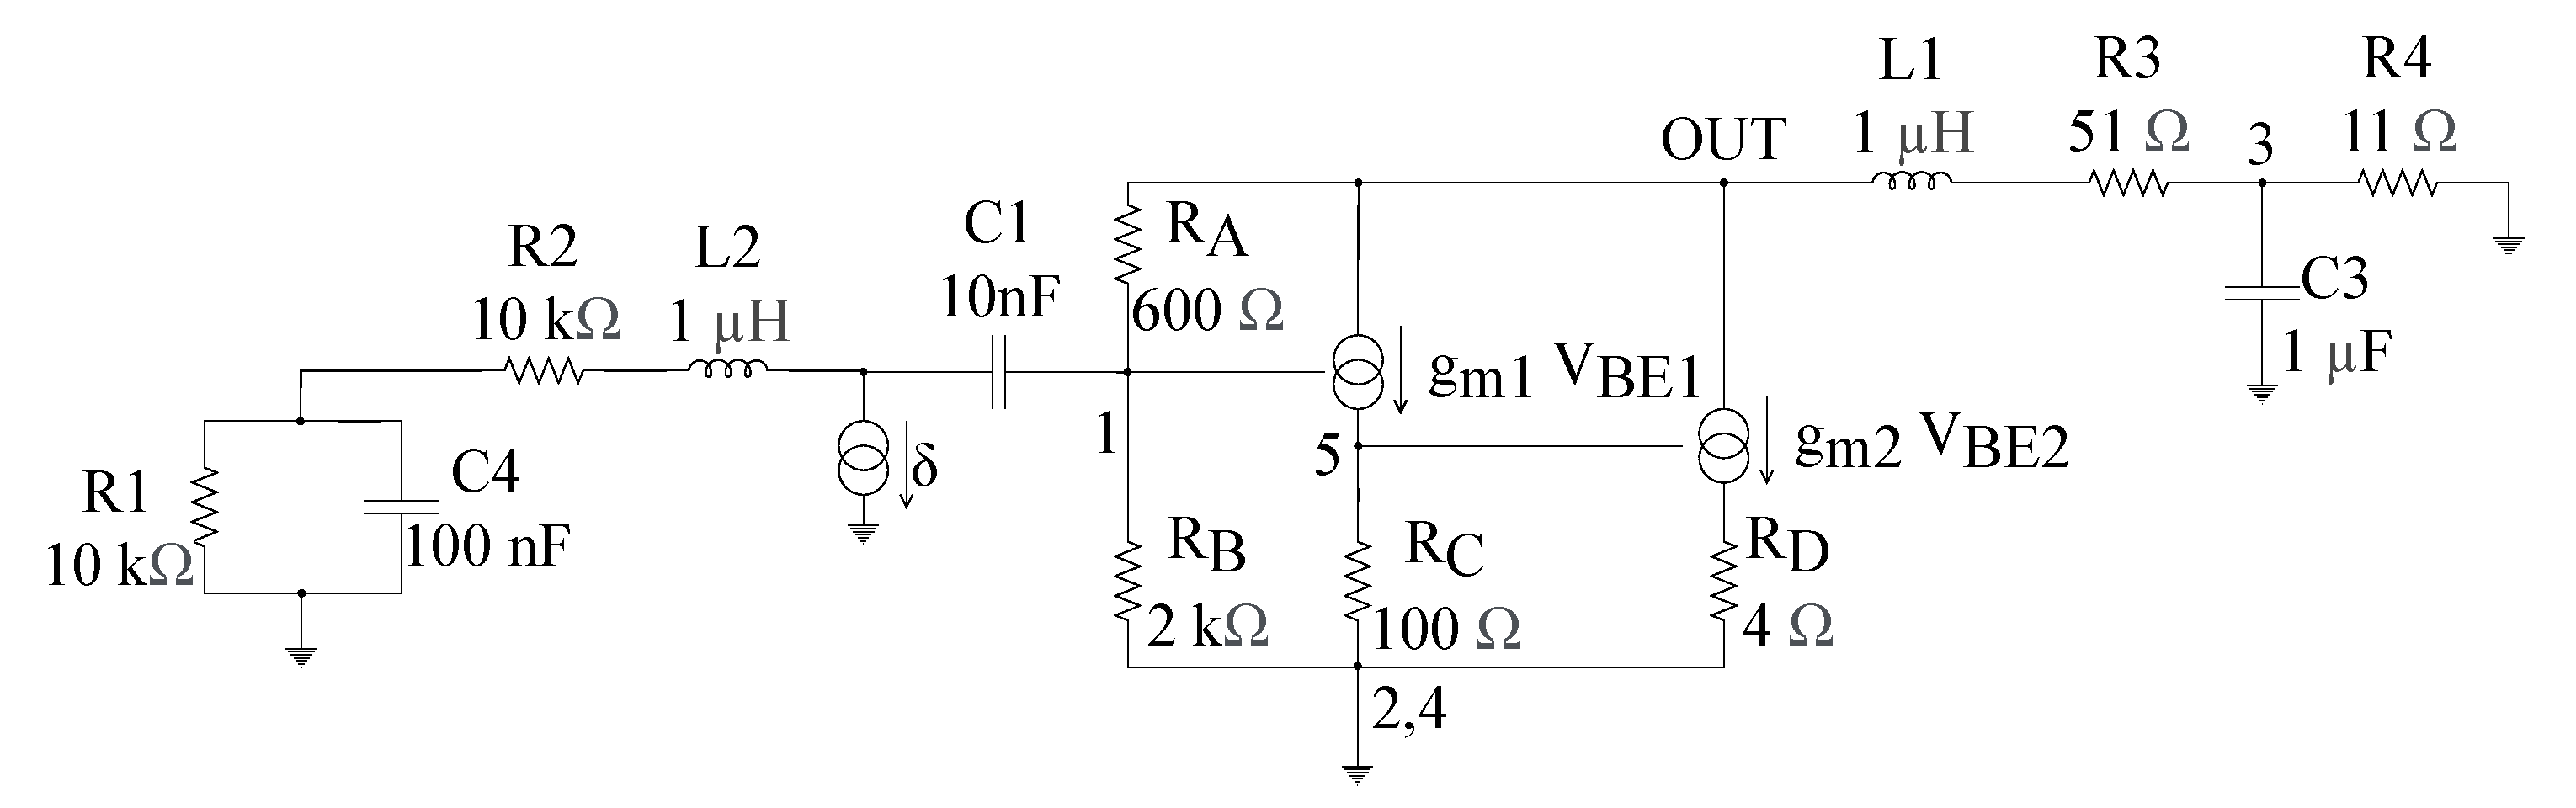
\includegraphics[width=1\linewidth]{img/preamp_circuito_ac.pdf}
    \caption{Schema circuitale del preamplificatore in AC.}
    \label{fig:preamp_circuito_ac}
\end{figure}

Osservando i valori degli induttori $L_1$ e $L_2$ e del condensatore $C_1$ e considerando che ci troviamo a frequenze dell'ordine dei 
\si{\giga\hertz}, possiamo assumere $\omega\to \infty$. Sapendo che per calcolare le impedenze induttive vale $Z_L=j \omega L$ e per quelle
capacitive $Z_C\frac{1}{j \omega C}$, è possibile modellizzare i condensatori come cortocircuiti e gli induttori come circuiti aperti trasformando il 
circuito come in \autoref*{fig:preamp_circuito_ac_senza_LC} e semplificando notevolmente i calcoli.
\begin{figure}[h!]
    \centering
    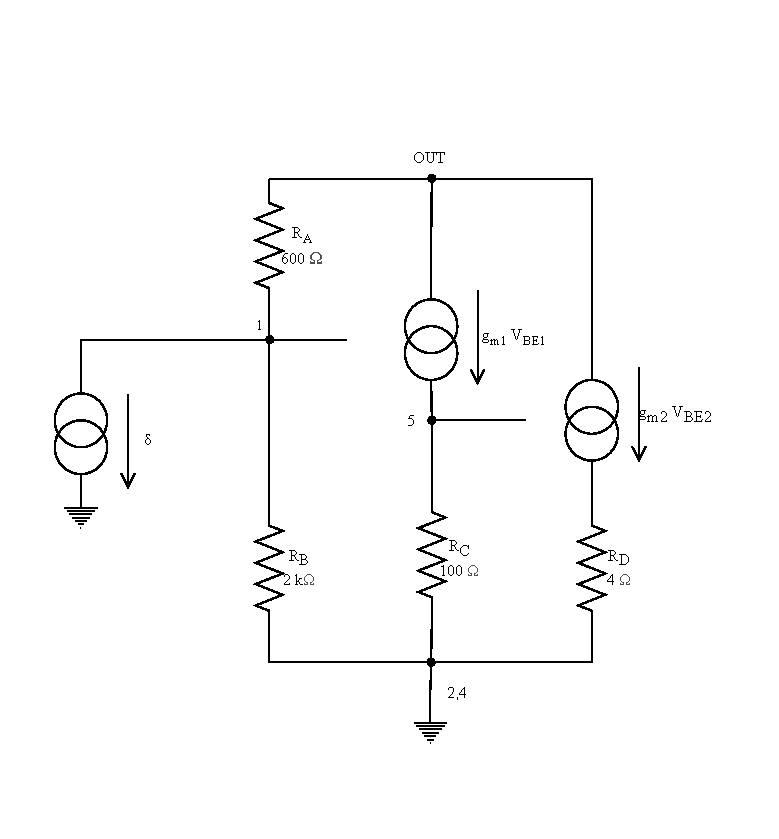
\includegraphics[width=1\linewidth]{img/preamp_circuito_ac_senza_LC.pdf}
    \caption{Schema circuitale del preamplificatore in AC considerando $\omega\to \infty$.}
    \label{fig:preamp_circuito_ac_senza_LC}
\end{figure}

Applicando al nodo 1la legge di Kirchoff ai nodi, si ottengono le \autoref*{eq:bilancio_nodo1}:
\begin{equation}
    \begin{gathered}
        i_A = \delta + i_B; \\
        \frac{V_\text{out} - V_1}{R_A} = \delta + \frac{V_1}{R_B}; \\
        V_1 = \frac{R_B V_\text{out} - R_A R_B \delta}{R_A + R_B}.
        \label{eq:bilancio_nodo1}
    \end{gathered}
\end{equation}
Osservando il circuito si nota che il transistor $Q_1$ si trova in configurazione di Emitter Follower, di conseguenza valgono le \autoref*{eq:emitter_follower}
\begin{equation}
    \begin{aligned}
        i_{\text{c}_1} &= g_{\text{m}_1} (V_{\text{B}_1} - V_{\text{E}_1});  \\
        &= g_{\text{m}_1} \left( V_1 - \frac{g_{\text{m}_1} R_1}{1 + g_{\text{m}_1} R_1} V_1 \right) \\
        &= g_{\text{m}_1} \frac{1}{1 + g_{\text{m}_1} R_1} V_1, \quad \text{con } g_{\text{m}_1} R_1 \gg 1 ;\\
        &= \frac{V_1}{R_1}.
    \end{aligned}
    \label{eq:emitter_follower}
\end{equation}
Infine, effettuando un bilancio di correnti al nodo $out$ otteniamo le \autoref*{eq:bilancio_nodo_out}:
\begin{equation}
    \begin{gathered}
        \delta + i_B + i_{\text{C}_1} + i_{\text{C}_2} = 0, \quad \text{dalla~\ref{eq:emitter_follower}} \\
        \delta + \frac{V_1}{R_B} + \frac{V_1}{R_C} + \frac{V_1}{R_D} = 0; \\
        \delta = -\left(\frac{1}{R_B} + \frac{1}{R_C} + \frac{1}{R_D}\right) V_1, \quad \text{con } R_D \ll R_C \ll R_B \\
        \delta = -\frac{V_1}{R_D}.
    \end{gathered}
    \label{eq:bilancio_nodo_out}
\end{equation}

Sostituendo poi \autoref*{eq:bilancio_nodo1} nella \autoref*{eq:bilancio_nodo_out} si ricavano le \autoref*{eq:finale}:
\begin{equation}
    \begin{gathered}
        \delta = -\frac{R_B}{R_D} \cdot \frac{V_\text{out} - R_A \delta}{R_A + R_B}; \\
        \frac{R_D}{R_B} \cdot (R_A + R_B) \delta = -V_\text{out}+R_A \delta; \\
        V_\text{out}=[R_A-R_D(1+\frac{R_A}{R_B})] \cdot \delta; \\
        V_\text{out}=R_A [1-R_D(\frac{1}{R_A}+\frac{1}{R_B})] \cdot \delta \\
    \end{gathered}
\label{eq:finale}
\end{equation}
Considerando che $R_D(\frac{1}{R_A}+\frac{1}{R_B})=0,0087 \ll 1;$, l'equazione finale è la \autoref*{eq:fdt}:
\begin{equation}
    V_\text{out}=R_A \delta
\label{eq:fdt}
\end{equation}
Si ottiene così la funzione di trasferimento che lega la corrente in uscita dal SiPM alla tensione in uscita dal preamplificatore. Un modo per 
verificare se i calcoli appena visti sono corretti è quello di confrontare il valore del guadagno della funzione di trasferimento ottenuto 
simulando il circuito con LTSpice con il valore del guadagno della \autoref*{eq:fdt}. Si verifica che 
$\left| \frac{V_{\text{out}}}{\delta} \right|_{\text{dB}}=\SI{55}{\dB}$. Per effettuare l'analisi in AC del circuito in \autoref*{fig:preamp_circuito} 
è sufficiente la direttiva \texttt{.ac dec 20 0.01 10G} 
con l'accortezza di assegnare al generatore di corrente $\delta$ il valore 1 con la direttiva \texttt{AC 1} dopo la sua definizione nella \texttt{netlist}.
La direttiva permette di visualizzare i diagramma di Bode della funzioni di trasferimento da $\delta$ al nodo selezionato. I parametri della direttiva
indicano che la simulazione resituirà 20 punti per decade da una frequenza di \SI{0.01}{\hertz} a una di \SI{10}{\giga\hertz}. Selezionando il nodo $3$, 
si ottengono i diagrammi nella \autoref*{fig:bode_preamp}.
Come si può osservare, il circuito si comporta come un filtro passa-alto con una frequenza di taglio $\omega_0 \approx \SI{8}{\kilo\hertz}$, avendo 
un guadagno crescente fino al valore $\omega_0$ per poi rimanere costante intorno al valore di \SI{55}{\dB}, concorde con quanto calcolato precedentemente.
Inoltre, osservando il diagramma della fase, si nota che diminuisce passando da \ang{90} a \ang{0}, andamento concorde a quello del filtro passa-alto.
Quindi, come previsto, il circuito preso in analisi si comporta come un amplificatore per alte frequenze.
\begin{figure}[h!]
    \centering
    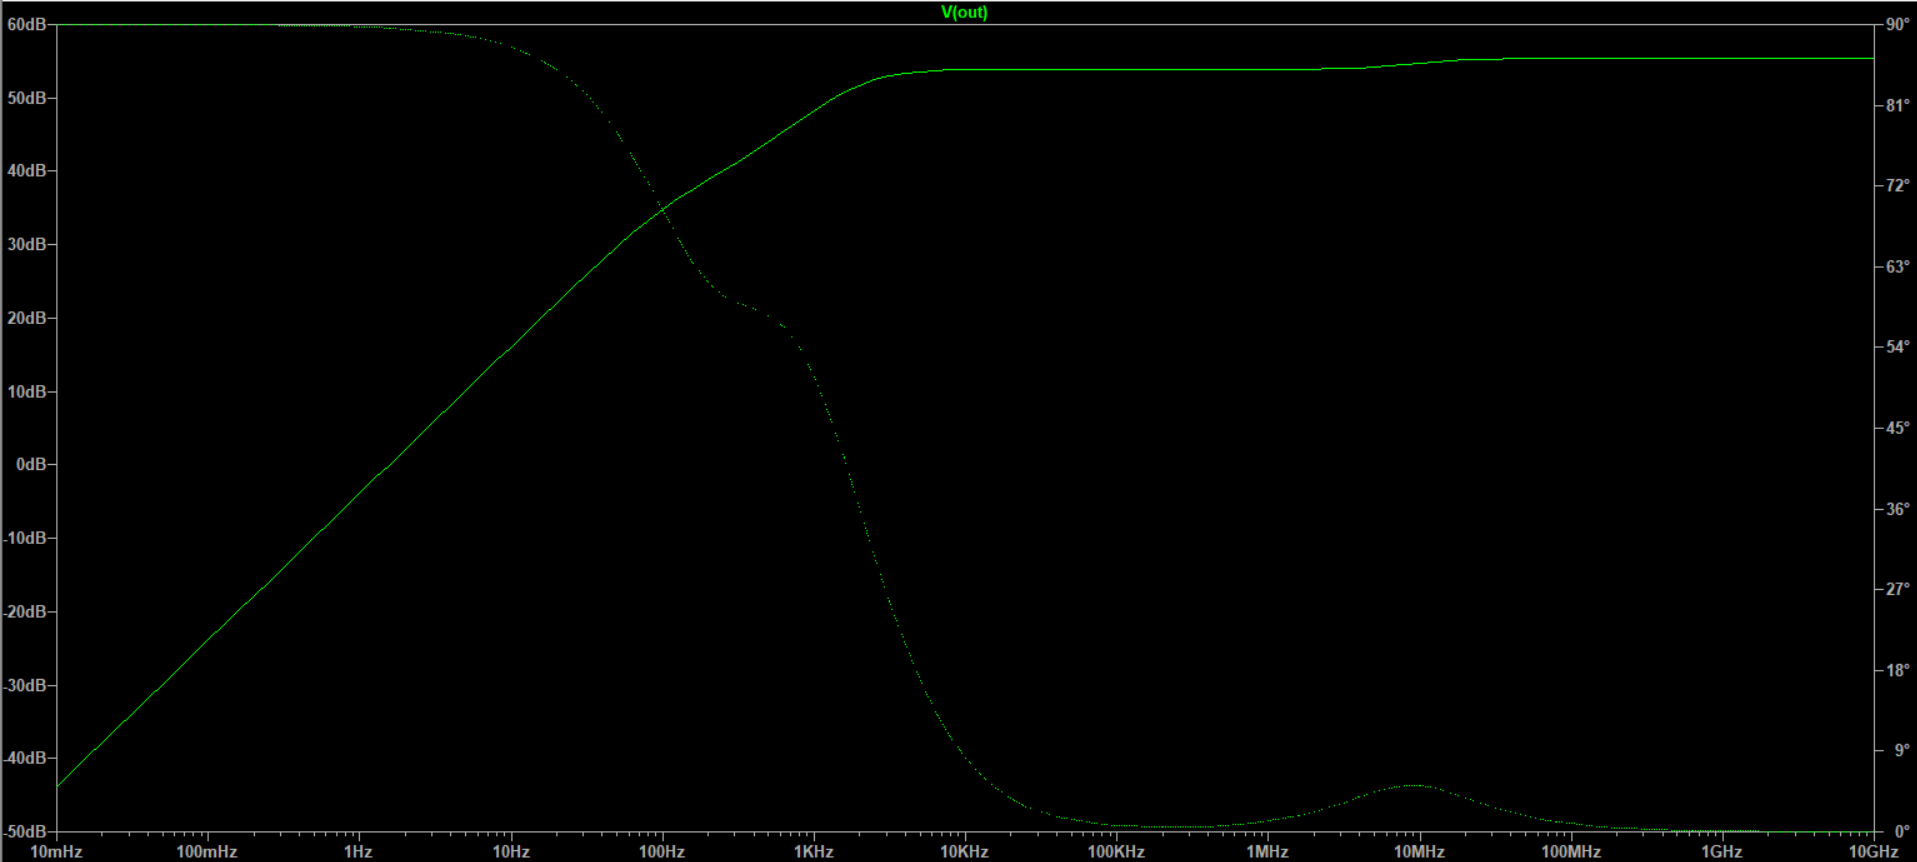
\includegraphics[width=1\linewidth]{img/bode_preamp.png}
    \caption{Diagrammi di Bode della funzione di trasferimento $\frac{V_\text{out}}{\delta}$. In linea continua il diagramma del guadagno, in linea
    tratteggiata quello della fase.}
    \label{fig:bode_preamp}
\end{figure}
\section{Analisi nel dominio del tempo}
Per capire come si comporta il circuito all'arrivo di un muone, occorre effettuare un'analisi detta in transitorio in cui si vuole ottenere 
l'andamento della tensione d'uscita in funzione nel tempo. Per farlo, usando LTSPice, è necessario modellizzare il comportamento del sottocircuito 
SiPM-scintillatore. Da dati raccolti empiricamente, in uscita dal sottocircuito si ha una corrente che segue un andamento a gradino, con un 
intervallo di tempo tra salita e discesa di circa una decina di nanosecondi e valore massimo dipendente dall'energia trasportata dal muone. 
Per modellizzare questo comportamento occorre scrivere, dopo la definizione del generatore di corrente $\delta$, \texttt{PULSE(0 {Id} 1n 1n 1n 9n)} 
che definisce un gradino con valore minimo di \SI{0}{\ampere}, valore massimo uguale a quello contenuto nella variabile \texttt{Id}, che verrà 
definita successivamente, ritardo rispetto l'inizio della simulazione di \SI{1}{\nano\second}, tempo di salita e discesa di \SI{1}{\nano\second} e 
tempo in cui il generatore eroga il valore massimo di corrente di \SI{9}{\nano\second}. La varabile \texttt{Id} è definita secondo la direttiva 
\texttt{.step param Id 0 20m 0.5m} secondo la quale la variabile assumerà tutti i valori compresi tra \SI{0} e \SI{20}{\milli\ampere} con 
un incremento di \SI{0,5}{\milli\ampere}. Per simulare l'andamento del circuito in transitorio la direttiva è \texttt{.tran 0 20n 0}: il software 
simulerà il circuito tra \SI{0} e \SI{2}{\nano\second} salvando i dati da \SI{0}{\second}. Selezionando il nodo $3$ nel circuito in 
\autoref*{fig:preamp_circuito}, si ottiene il grafico della \autoref*{fig:out_tran_0_20m}. Come si può vedere, il circuito, per certi 
valori di corrente ha un andamento difficile da definire. È utile allora in questo caso stabilire la caratteristica I-V che lega la corrente in 
ingresso alla tensione in uscita. Dal grafico si vede che il valore della tensione d'uscita dipende dall'istante di tempo e dal valore della 
corrente in ingresso. Non potendo rappresentare la tensione con entrambi i parametri, si è deciso di rappresentare la caratteristica I-V a \SI{7}{\nano\second}. 
Il motivo è che il valore si trova circa a metà del tempo di corrente massima. Per fare ciò,
occorre scrivere la direttiva \texttt{.meas TRAN result FIND V(out) AT 7n}, si ottiene così il grafico della \autoref*{fig:caratteristica_IV_preamp_0_20m}.
\begin{figure}[h!]
    \centering
    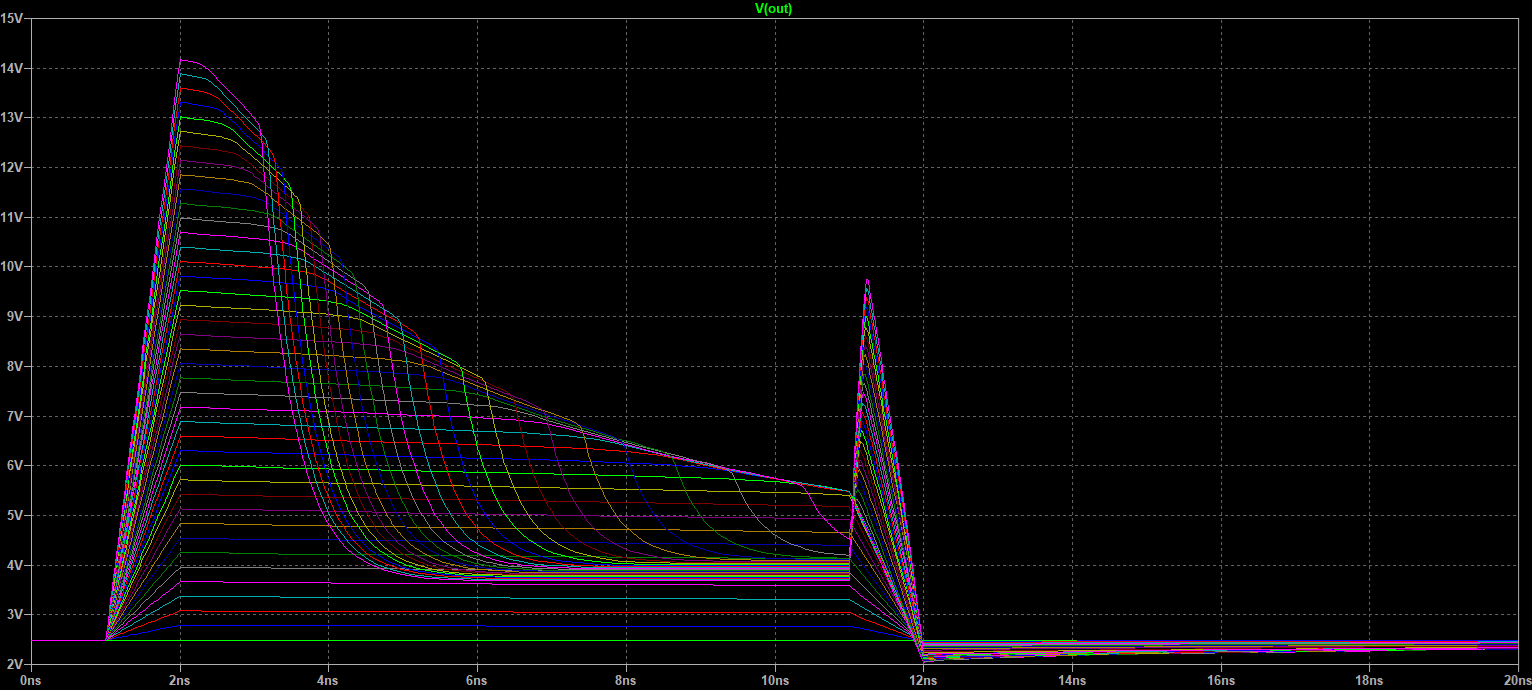
\includegraphics[width=.65\linewidth]{img/out_tran_0_20m.png}
    \caption{Andamento in transitorio del nodo $3$ del preamplificatore.}
    \label{fig:out_tran_0_20m}
\end{figure}
\begin{figure}[h!]
    \centering
    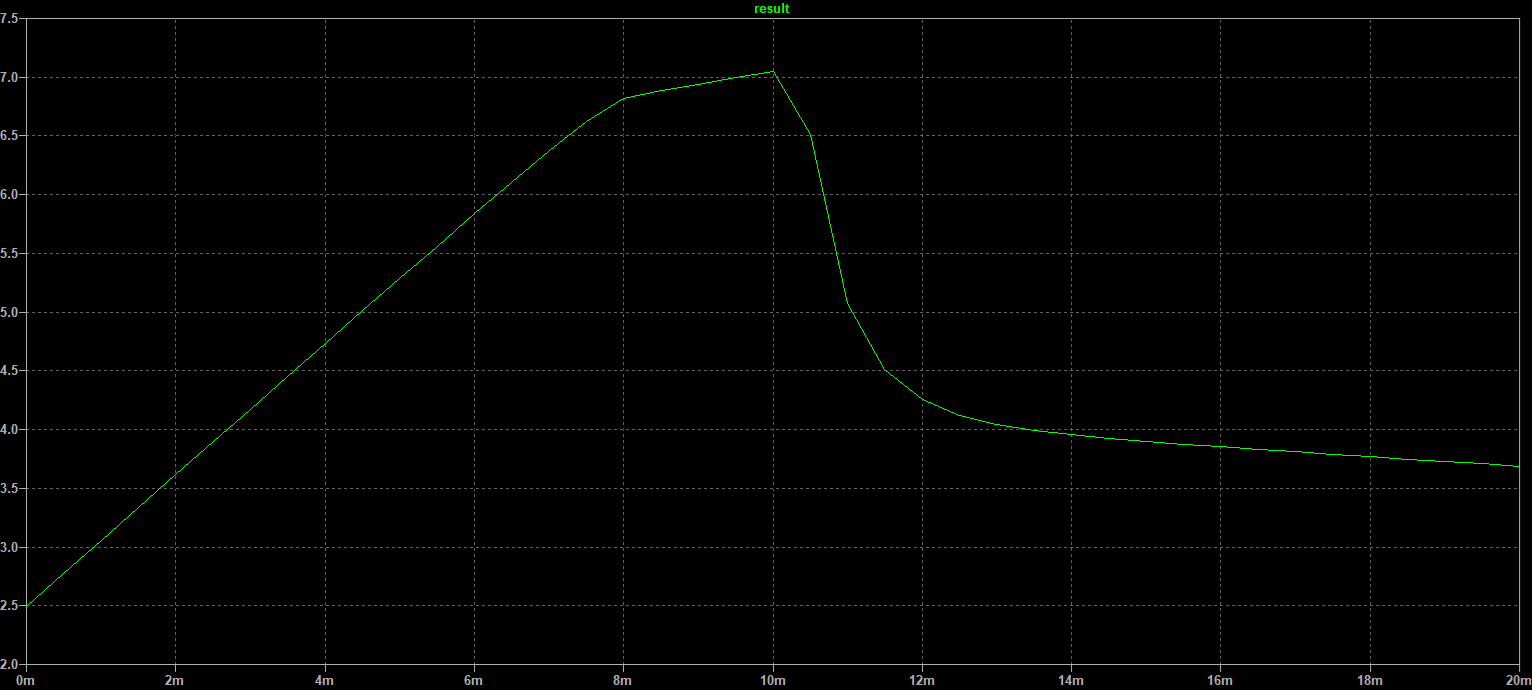
\includegraphics[width=.65\linewidth]{img/caratteristica_IV_preamp_0_20m.png}
    \caption{Caratteristica I-V del preamplificatore per valori di corrente compresi tra \SI{0}{\ampere} e \SI{20}{\milli\ampere}.}
    \label{fig:caratteristica_IV_preamp_0_20m}
\end{figure}

Osservando il grafico si nota un andamento lineare tra \SI{0} e \SI{8}{\milli\ampere}. Questa è la zona di interesse, in cui il circuito
ha l'andamento migliore per svolgere poi eventuali elaborazioni sui dati ottenuti. È lecito, infatti, aspettarsi una proporzionalità diretta tra 
l'energia trasportata dal muone e il valore di tensione in uscita dal preamplificatore. Restringendo quindi il grafico della \autoref*{fig:caratteristica_IV_preamp_0_20m}
tra \SI{0}{\ampere} e \SI{8}{\milli\ampere} si ottiene il grafico della\autoref*{fig:caratteristica_IV_preamp_0_8m}. Calcolando il valore del 
coefficiente angolare dal grafico si ottiene $m=\SI{600}{\volt/\ampere}=R_A$, come previsto dall'analisi del circuito in AC.
\begin{figure}[h!]
    \centering
    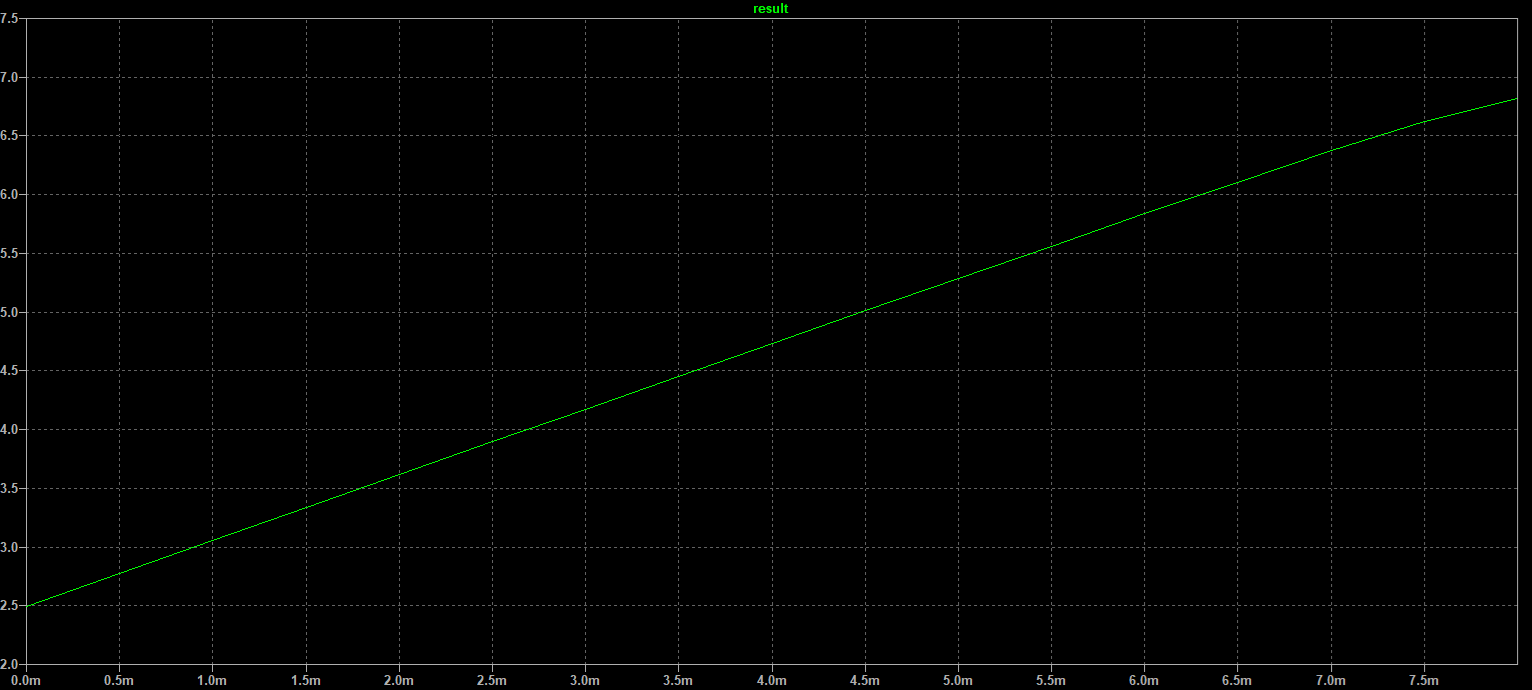
\includegraphics[width=.65\linewidth]{img/caratteristica_IV_preamp_0_8m.png}
    \caption{Caratteristica I-V del preamplificatore per valori di corrente compresi tra \SI{0}{\ampere} e \SI{8}{\milli\ampere}.}
    \label{fig:caratteristica_IV_preamp_0_8m}
\end{figure}
\section{Progettazione della PCB}
Le simulazioni e i calcoli visti sono utili per comprendere il funzionamento del circuito e facilitare la sua realizzazione. Per poter utilizzare il
circuito preso in esame è necessario progettare la Printed Circuit Board (PCB) o circuito stampato. Un circuito stampato è un supporto
usato per connettere i componenti di un circuto tramite dei conduttori, chiamati piste, incisi su un materiale non conduttivo.
Per fare ciò si è utilizzato EAGLE, un software, distribuito da Autodesk, facente parte della categoria di strumenti per progettare e produrre
sistemi elettronici (EDA, ossia Electronic Design Automation). 
Questo software permette ai progettisti di PCB di connettere tra di loro lo schematico del circuito, il posizionamento delle compenenti e il PCB 
routing, cioè il collegamento dei componenti.

La prima fase dello sviluppo di una PCB con EAGLE è la realizzazione dello schematico. Nel caso preso in esame, lo schematico appare come nella
\autoref*{fig:schematico_pcb}. Rispetto al circuito della \autoref*{fig:preamp_circuito}, si ha la presenza di quattro componenti con il 
prefisso JP e l'assenza dei generatori di tensione e di quello di corrente. I generatori di tensioni mancano perché non è possibile collocarli sulla
PCB; ma è necessario fornire l'alimentazione dall'esterno. Il generatore di corrente era un modello per descrivere
il comportamento del sottocircuito SiPM-scintillatore, che, come i generatori di tensione, può essere visto come collegato dall'esterno. Per connettere
dei dispositivi tra loro è necessario disporre dei connettori, indicati nello schematico proprio dal prefisso JP. In particolare, il connettore
JP1 connette il SiPM-scintillatore al preamplificatore attraverso il morsetto 1 e riceve le tensioni di alimentazione per il SiPM dai connettori
2 e 3. Il connettore JP2 fornisce ancora l'alimentazione al circuito, il connettore JP3 è connesso ai generatori di tensione e il connettore JP4
riceve la tensione del nodo di uscita.
\begin{figure}[h!]
    \centering
    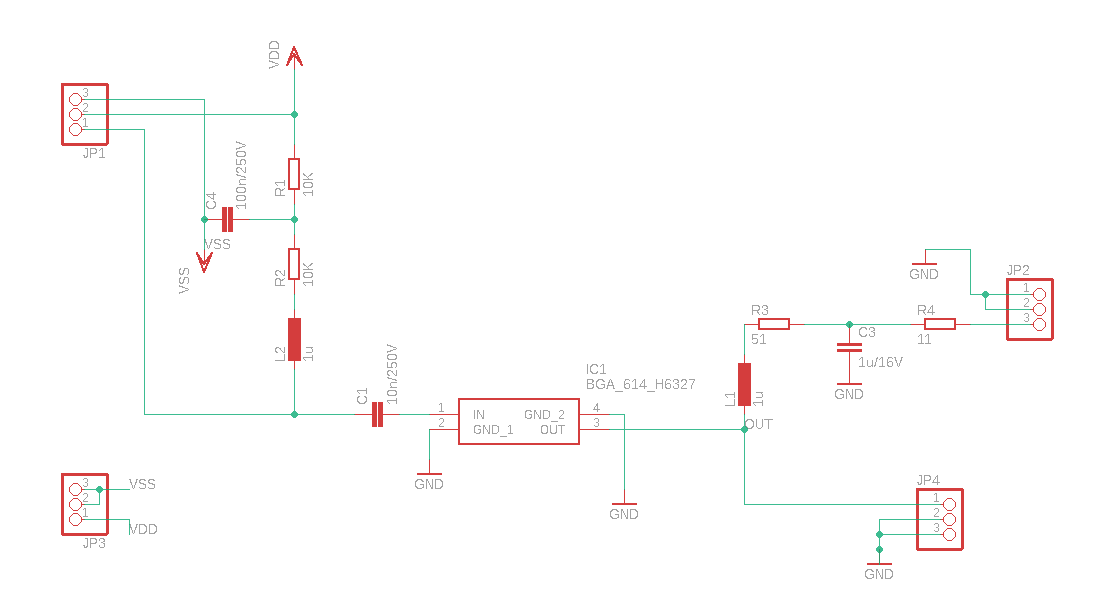
\includegraphics[width=\linewidth]{img/schematico_pcb.png}
    \caption{Schematico del preamplificatore in EAGLE.}
    \label{fig:schematico_pcb}
\end{figure}
Disegnando lo schematico è necessario decidere quale modello del dispositivo, se sono presenti diverse opzioni, montare. Nel caso preso in esame, i componenti su
cui c'era più possibilità di scelta erano i resistori, i condensatori e gli induttori. Per ognuno dei tre componenti  è possibile scegliere il tipo di 
montaggio tra due modalità: PTH o SMD. PTH è un acronimo che sta per Pass Through Hole e indica che i dispositivi assemblati in questa 
maniera sono dotati di piedini che vengono inseriti in alcuni fori presenti nella PCB e saldati dalla parte opposta della 
scheda. SMD, invece, significa Surface Mounted Device; in questa categoria rientrano i dispositivi che possono venire saldati sullo stesso 
lato in cui vengono montati senza avere nessun piedino e nessun foro nella PCB. Quest'ultimi dispositivi, inoltre, sono più piccoli e 
hanno prestazioni migliori a frequenze pari a quelle che si hanno nel caso di studio trattato. Per avere una visione più chiara della differenza 
tra PTH e SMD si può osservare la \autoref*{fig:diff_pth_smd}.
\begin{figure}[h!]
    \centering
    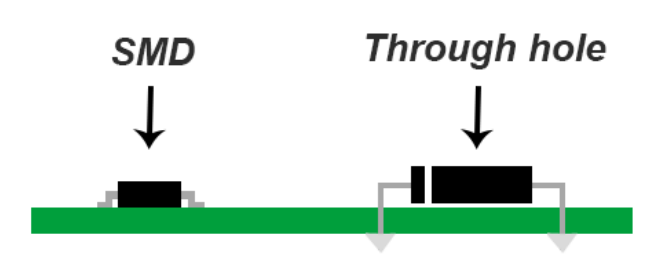
\includegraphics[width=.65\linewidth]{img/diff_pth_smd.png}
    \caption{Differenza visiva tra dispositivi SMD, a sinistra, e dispositivi PTH, a destra.}
    \label{fig:diff_pth_smd}
\end{figure}
Nel caso preso in analisi, per le considerazioni appena fatte, tutti i dispositivi tra resistori, capacitori e induttori usati sono di tipo SMD.
Una volta completato lo schematico, è buona prassi effettuare l'ERC (Electrical Rule Check) un controllo del software che verifica se sono presenti
eventuali errori elettrici nel circuito, come per esempio l'assenza di una massa.

Dopo aver completato il disegno dello schematico e effettuato l'ERC, EAGLE genera automaticamente il layout della board. La prima 
cosa da fare è decidere da quanti layer sarà formata la PCB. In questo caso, la PCB avrà 2 layer. Dopo aver scelto i layer, si devono 
impostare le regole di progetto da definire in base alla capacità produttiva seguendo le linee guida del produttore. Da qui inizia la fase 
di design in cui si devono collocare i componenti inseriti nello schematico all'interno del layout con l'accortezza di disporre vicini i 
dispositivi che saranno connessi l'uno con l'altro. Questo permette di ridurre le dimensioni della board. Tuttavia, non si devono collocare i dispositivi troppo vicini per evitare di avere disturbi dovuti ad 
interferenze. Una volta posizionati i componenti, si possono connettere tra loro con le piste. È stata scelta una larghezza delle piste
pari \SI{0.3048}{\milli\meter} per avere la possibilità di far scorrere nel circuito un corrente elevata.
Normalmente, si collegano prima i segnali, poi le alimentazioni ed infine le masse. Nel tracciare le piste bisogna assolutamente evitare gli angoli
di \ang{90} perché questi fanno perdere integrità al segnale, creano cioè rumore, e aumentano la probabilità di errori di fabbricazione. Come per la collocazione dei 
componenti, va lasciato spazio tra piste, dispositivi, eventuali via e fori metallizzati usati per interconnettere due o più layer della board.
I via sono importanti perché permettono una miglior distribuzione della potenza e del segnale di massa, è norma aggiungerli dove sono presenti
ampie aree prive di componenti o via.

Dopo aver tracciato tutte le piste è necessario creare il piano di massa. Analogamente a quanto effettuato con lo schematico, anche per il layout
si effettua un controllo chiamato DRC (Design Rule Check) dove si verifica che siano state rispettate le regole del progetto. 
La PCB progettata per il preamplificatore è riportata in \autoref*{fig:preamp_board}: si può notare l'assenza di angoli retti, la vicinanza dei dispositivi collegati
tra loro e la presenza dei via in zone ampie senza componenti o piste.
\begin{figure}[h!]
    \centering
    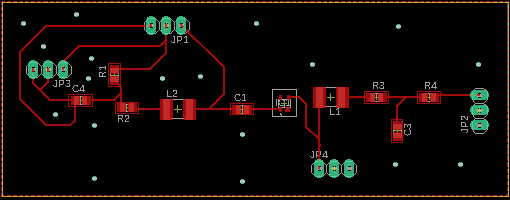
\includegraphics[width=.65\linewidth]{img/preamp_board.png}
    \caption{La PCB dell'amplificatore. Le dimensioni sono di $\SI{85.8}{\milli\meter} \times \SI{33.3}{\milli\meter}$}
    \label{fig:preamp_board}
\end{figure}

Riassumendo, in questa parte di lavoro, lo studio del preamplificatore è iniziato con l'analisi del dispositivo elettronico BGA614, componente fondamentale del circuito, di cui poi 
è stata fatta un'analisi completa. Il calcolo del punto di lavoro stazionario ha permesso di conoscere lo stato dei componenti attivi del circuito,
l'analisi di piccolo segnale ha stabilito il comportamento del circuito alle frequenze operative del sottocircuito SiPM-scintillatore e l'analisi 
in transitorio ha messo in luce la reazione del circuito all'arrivo dei segnali dal sottocircuito. Queste tre analisi hanno coperto tutti i domini
operativi di un circuito, prevedendo così il suo comportamento. Infine, la progettazione della PCB ha realizzato il design costitutivo del circuito
rendendolo pronto alla fabbricazione per poi essere utilizzato nel campo di applicazione descritto da questo lavoro.